\chapter{Introduction}

This manual aims to guide end users in the application of InVesalius tools and also presents some concepts to facilitate the use of the software.

InVesalius is software that is designed to assist health professionals on diagnosis and surgical planning. It should be noted, however, that all software in the diagnostic context is fully supplementary, and each and every act committed is the responsibility of health professionals.
 
In addition to medicine, InVesalius can be utilized in other areas such as archeology, medicine, dentistry, veterinary, or even in industrial applications. As a basic requirement, the images to be analyzed are in DICOM (Digital Imaging Communications in Medicine). To date, InVesalius reconstructs images stemmed from CT scanners and MRI machines. To operate the software, basic computer literacy is essential. Understanding medical images can help to form a better understanding of the operations.

\section{Important Concepts}

Detailed in this section are a list of concepts essential to better understand and operate the software.

\subsection{DICOM (\textit{Digital Image Communications in Medicine})}	

DICOM is a standard the transmission, storage and treatment of medical images. The standard encompasses various origins of medical images, such as images emanating from computed tomography (CT) equipment, magnetic resonance, ultrasound, and electrocardiogram, among others.

A DICOM image consists of two main components, namely, an array containing the pixels of the image and a set of meta-information. This information includes, but is not limited to, patient name, mode image and the image position in relation to the space (in the case of CT and MRI).

\subsection{Computed Tomography - Medical}

Computed tomography indicates the radiodensity of tissues, i.e., the average X-ray absorption by the tissues. The radiodensity reading is translated into an image gray levels, called the Hounsfield scale, named Godfrey Newbold Hounsfield, one of the creators of the first CT scan.

\begin{figure}[!htb]
\centering
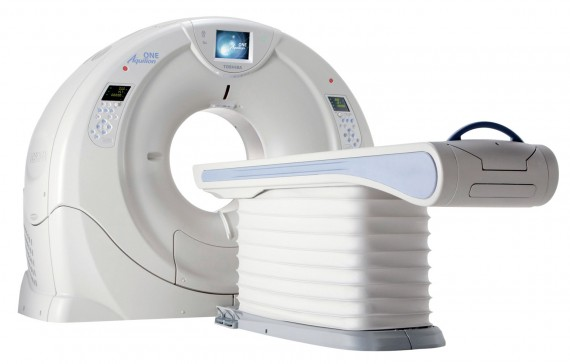
\includegraphics[scale=0.4]{../user_guide_figures/tomografo.jpg}
\caption{Medical CT scanner - www.toshibamedical.com.br}
\end{figure}

Most modern CT scanning appliances are equipped with a radiation emitter and a sensor bank (with channels ranging from 2 to 256), which circle the patient while the stretcher is moved, forming a spiral. This generates a large number of images simultaneously, with little emission of X-rays.

\subsubsection{Hounsfield Scale}

As mentioned in the previous section, the CT images are generated in gray levels, expressed in Hounsfield (HU), wherein lighter shades represent denser matters, and the darker, less dense matter such as skin and brain tissues. 

Table~\ref{tab:escala_hounsfield} presents some materials and their respective values in Hounsfield Units (HU).

\begin{table}[h]
\centering
\caption{Escala de Hounsfield}
\begin{tabular}{lcc}\\
\hline % este comando coloca uma linha na tabela
Material & HU\\
\hline
\hline
Air & -1000 or less\\
Fat & -120\\
Water & 0\\
Muscle & 40\\
Contrast & 130\\
Bone & 400 or more\\
\hline
\end{tabular}
\label{tab:escala_hounsfield}
\end{table}


\subsection{Computed Tomography - Dental (CBCT)}

The dental CT commonly works with less radiation emission compared to medical CT, and therefore makes it possible to view more details of delicate regions such as alveolar cortical.

\begin{figure}[!htb]
\centering
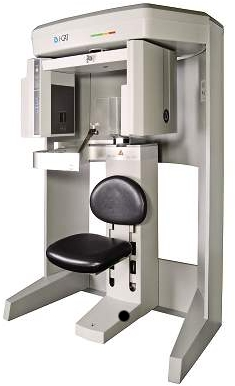
\includegraphics[scale=0.4]{../user_guide_figures/feixe_conico.jpg}
\caption{Dental tomography - www.kavo.com.br}
\end{figure}

Image acquisition is performed with the patient positioned vertically (as opposed to medical tomography in which the patient is horizontal). A transmitter X-ray surround the patient's skull, forming an arc of $180^\circ$ or $360^\circ$. The images generated are compiled as a volume of the patient's skull. This volume is then "sliced" by the software into individual layers, being able to generate images with different spacing or fields of view, such as a panoramic view of the region of interest.

The images acquired by dental scanners often require more post processing when it is necessary to separate (segmental) certain structures using other software such as InVesalius. This is because, typically, these images have more gray levels than, which makes use of segmentation patterns (preset) less. Another very common feature in the images of provincial dental CT scanners is the high presence of speckle noise and other forms of noise typically caused by the presence of amalgam prosthetics.

\subsection{Magnetic Resonance Imaging - MRI}

MRI is an examination performed without the use of ionizing radiation. Instead, it use a strong magnetic field to align the atoms of any element present in our body, most commonly hydrogen. After alignment, radio waves are triggered to excite atoms. The sensors measure the time that the hydrogen atoms take to realign. This makes it possible to distinguish between different tissues, as different types possess different quantities of hydrogen atoms.

To avoid interference and improve the quality of the radiofrequency signal, the patient is placed inside a narrow tube encompassed by the coil and scanning unit.

\begin{figure}[!htb]
\centering
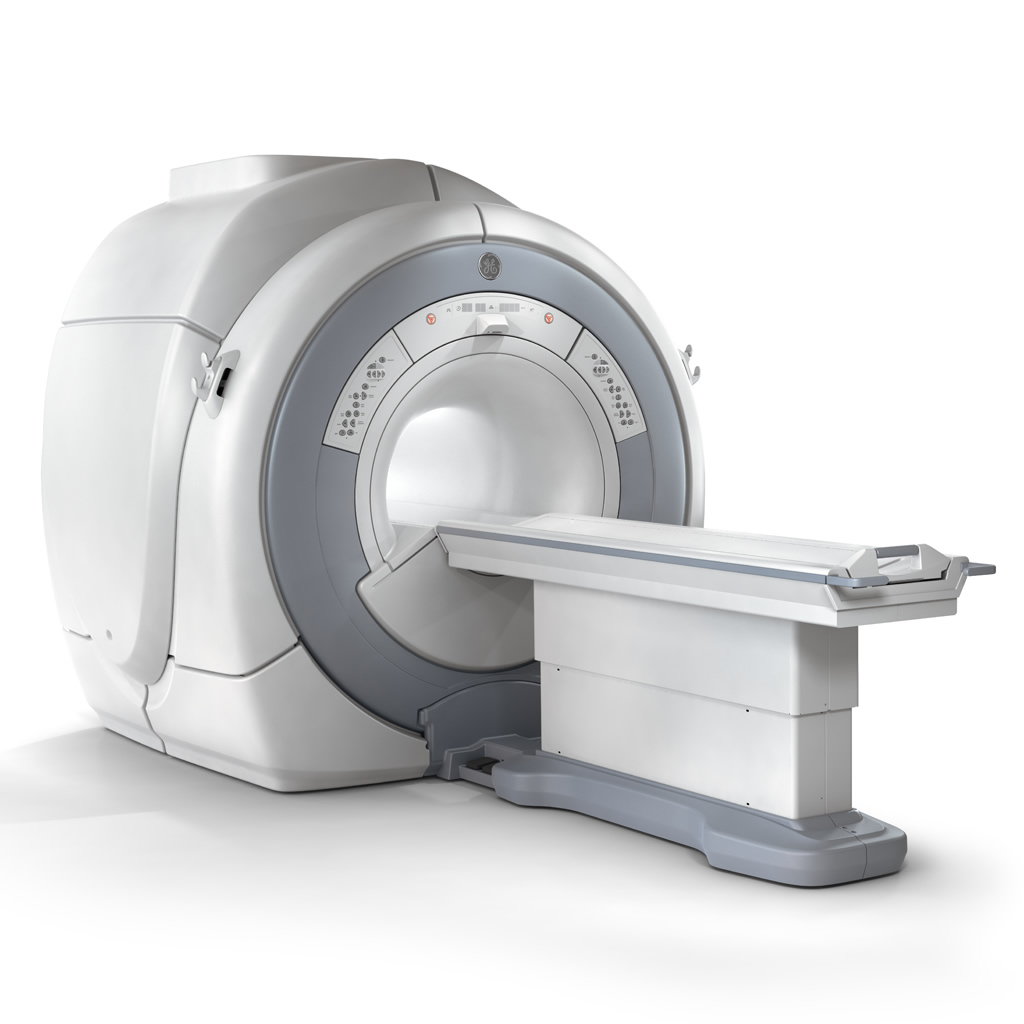
\includegraphics[scale=0.2]{../user_guide_figures/rm_ge.jpg}
\caption{Magnetic resonance imaging equipment - www.gehealthcare.com}
\end{figure}

\begin{figure}[!htb]
\centering
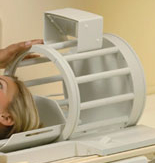
\includegraphics[scale=0.8]{../user_guide_figures/bobina.jpg}
\caption{Coil - www.healthcare.philips.com}
\end{figure}

\subsection{Neuronavigation}
\label{sec:neuronavegador_intro}

Neuronavigation is a technique that allows tracking and localization of surgical instruments relative to neuronal
structures through computer visualization. In addition, neuronavigation systems a fundamental tool to aid surgical plan and to increase the accuracy of experiments in neuroscience, such as transcranial magnetic stimulation (TMS), electroencephalography (EEG), magnetoencephalography (MEG) and near-infrared spectroscopy (NIRS).
Despite the vast field of applications, the use of neuronavigation in research centers is limited by its high cost.
InVesalius Navigator offers users a low-cost, open-source alternative to commercial neuronavigation systems. In this sense, it is possible to use specific tools for
neuronavigation and still have the possibility of developing features on demand. The software for neuronavigation is distributed in an executable version compatible with Windows 7, 8 and 10 operating system. The chapter~\ref{sec:neuronavegador} goes into details of all features of neuronavigation in InVesalius.

\section{Resources needed}

InVesalius is designed to run on personal computers, such as desktops and notebooks. Currently, it is compatible with the following operating systems:

\begin{itemize}
	\item Microsoft Windows (Windows 7, 8, 10)
	\item GNU/Linux (Ubuntu, Mandriva, Fedora) 
	\item Apple Mac OS X
\end{itemize}

The performance of InVesalius depends mainly on the amount of reconstructed slices (images offered by the software), the amount of random access memory (RAM) available, the processor clock rate \& frequency, and operating system architecture (32-bit or 64-bit).

It is important to note that, as a general rule, the greater the amount of RAM available on the system, the greater the number of slices that can be opened simultaneously. For example, with 1 GB of available memory, it can open about 300 slices with a resolution of 512x512 pixels. With 4 GB of memory, around 1000 images can be opened simultaneously at the same resolution.

\subsection{Minimum settings}

\begin{itemize}
	\item 32-bit Operating System
	\item Intel Pentium 4 or equivalent 1.5 GHz
	\item 1 GB of RAM
	\item 10 GB available hard disk space
	\item Graphics card with 64 MB memory
	\item Video resolution of 1024x768 pixels
\end{itemize}


\subsection{Recommended settings}
\begin{itemize}
	\item 64-bit Operating System
	\item Intel Core 2 Duo processor or equivalent 2.5 GHz
	\item 8 GB of RAM
	\item 20 GB available hard disk space
	\item NVidia or ATI graphics card with 128 MB of memory
	\item Video resolution of 1920x1080 pixels
\end{itemize}


